\section{Data Reduction}
% description of how reduced and calibrated  your data

The CCD observations are registered as astronomical images (FITS, Flexibble
Image Transport System). All the
analysis was done in IDL and ATV \cite{atv} - the source codes are
included in the appendix.




\subsection{CCD Dark Frame Calibration}

The first step of the data reduction is to remove the various instrumental
artifacts of the CCD, by calibrating  the science images. We create {\it dark
master frames} for every exposure times, \ie median combined frames of the CCD
closed, the high signal-to-noise dark. We subtract these frames from the
respective science frames with same exposure times and median combine these
last to form a deep exposure frame.


\subsection{Spectra Trace Calibration}

Spectra are arranged on the CCD in a manner that most efficiently makes
use of the detector size/area. Before these spectra can be extracted, their
exact positions on the CCD must be mapped. This is the process of {\it 
aperture tracing}. To this, we calculated the  spectra's {\it trace} from two
methods:
\begin{enumerate}
 \item Method 1: From a standard point source;
\item Method 2: By integrating the 1 + 1/2 strips.
\end{enumerate}

The trace of the point source, \eg a bright
(standard) star in the sky, is taken by positioning this star in each of the
three slits.
With ATV \cite{atv}, it is possible to extract the {\it spectral flux
distribution} \footnote{Loading the image with \texttt{decomposed, device=0}
option and pressing \texttt{x} on it.}, $F_{\lambda}$,  as shown in the Fig.
\ref{f}.

\begin{figure}[htb]
\begin{center}
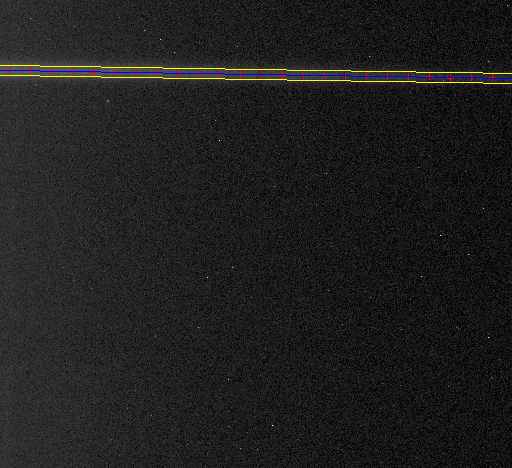
\includegraphics[scale=0.25]{plots/trace/point2.png}
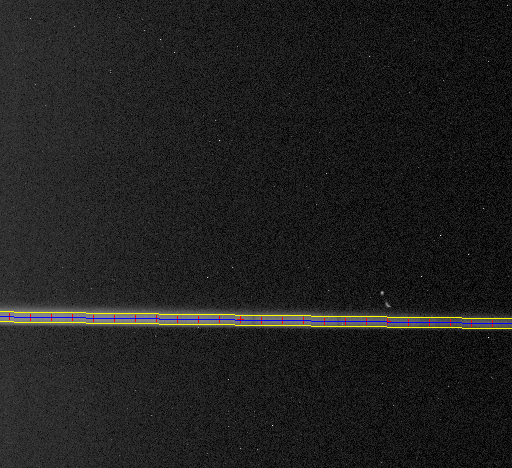
\includegraphics[scale=0.25]{plots/trace/point3.png}
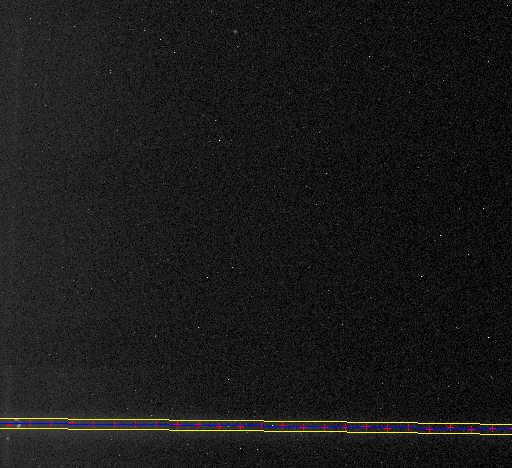
\includegraphics[scale=0.25]{plots/trace/point1.png}
\caption{Trace extraction from a point source  star in each of the three
slits
(from ATV).}
\label{f}
\end{center}
\end{figure}

 For the Moonshine, the flux is very high and using only the the point
source trace (method 1) was enough.
(see Figs. \ref{star-cal}).



\begin{figure}[htb]
\begin{center}
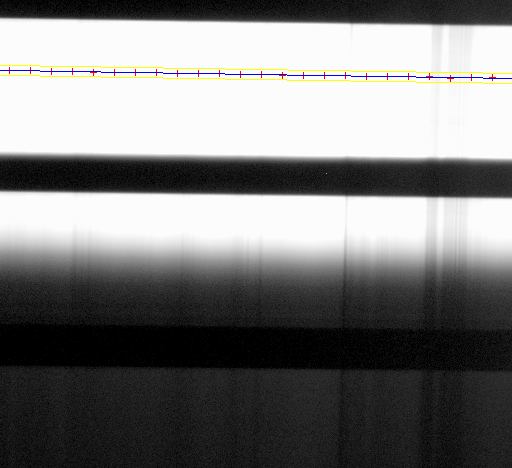
\includegraphics[scale=0.33]{plots/trace/moon.png}
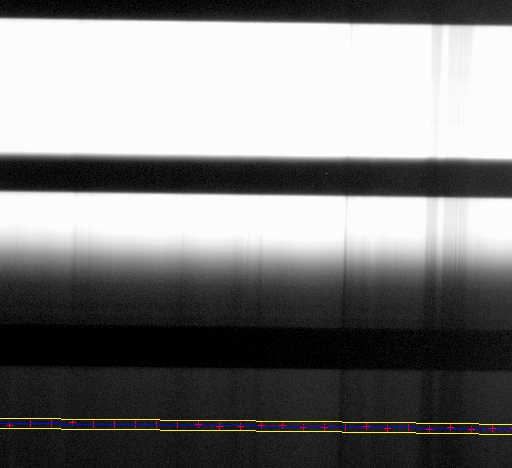
\includegraphics[scale=0.33]{plots/trace/moonsky.png}
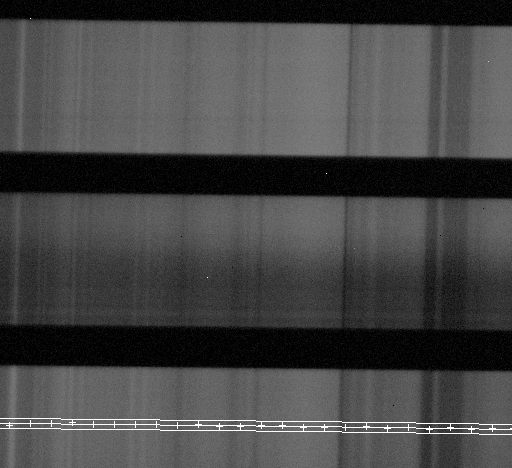
\includegraphics[scale=0.33]{plots/trace/earth.png}
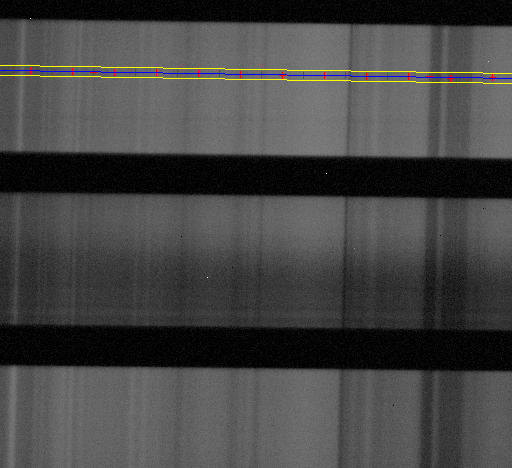
\includegraphics[scale=0.33]{plots/trace/earthsky.png}
\caption{Extraction of the point source spectra for the bright (above) and dark
(below) side of the
waning crescent moon and its adjacent sky (from ATV).}
\label{star-cal}
\end{center}
\end{figure}


Only for the Earthshine, due
to their much lower signal (in the same order of the adjacent sky), we determine
a second set of data (method 2), aiming to extract more statistics from the
data. We proceeded integrating over the whole
Earthshine strip and adding half of the middle strip (which has the adjacent
sky on the other half).





\subsection{Adjacent Sky Subtraction}
Both the dark and bright side of the Moon are corrected for scattered
light in the telescope by subtracting the adjacent sky spectrum. The adjacent
skies were always extracted in the same way the their respective set of data. The
sky-subtracted spectra can been in the see Figs. \ref{comparing}. 



\begin{figure}[htb]
\begin{center}
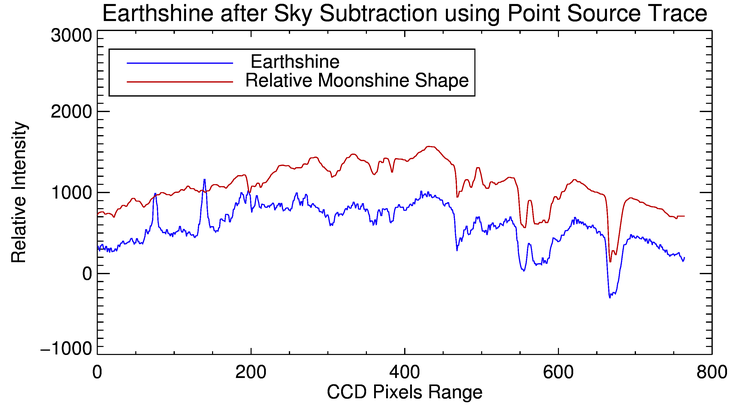
\includegraphics[scale=0.31]{plots/earth_point.png}
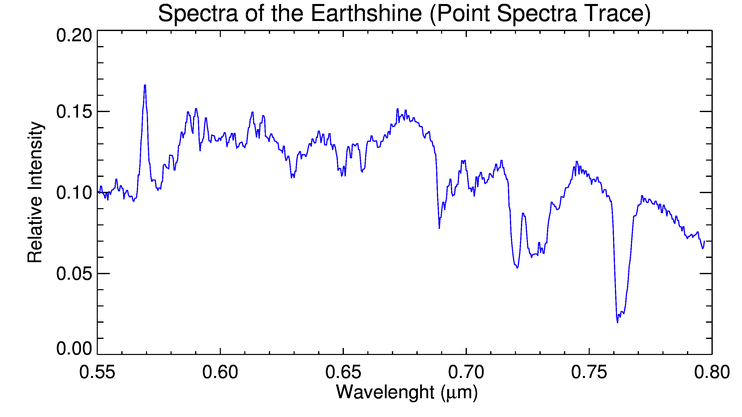
\includegraphics[scale=0.31]{plots/spectra1.png}
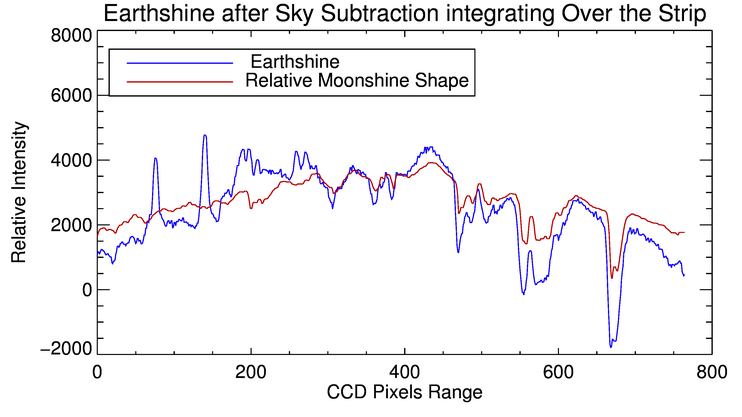
\includegraphics[scale=0.31]{plots/earth_strip.png}
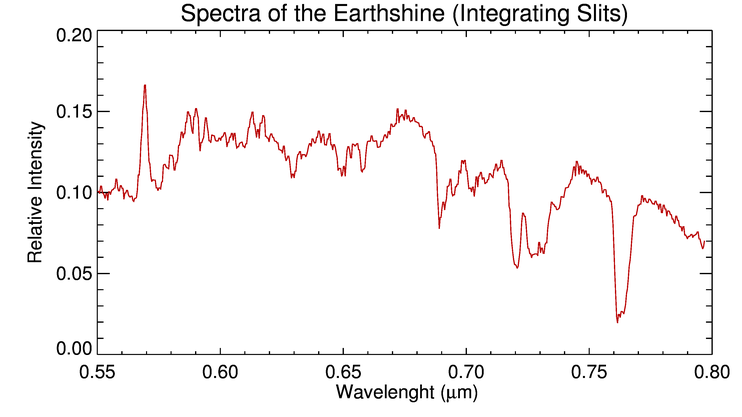
\includegraphics[scale=0.31]{plots/spectra2.png}
\caption{Earthshine spectra from method 1(top) and method 2 (down), comparing
to the scaled Moonshine spectra, in function of CCD pixel counts, and
wavelength calibrated.}
\label{comparing}
\end{center}
\end{figure}

After these
reductions we were able to calculate the signal
to background for
the Earthshine (methods 1 and 2) and for the Moonshine spectra, obtaining
$S/N^{point}_{earth} = 1.8$,  $S/N^{strip}_{earth} = 3.4$ and
$S/N_{moon} = 148$, respectively.

\subsection{Obtaining the Reflectivity of Earth}


The reflectivity of Earth is the ratio of the Earthshine to the Moonlight
spectra, \ie by reducing the contribution of the extra
passage of the Sun through the Earth's atmosphere in the spectrum of the
Earthshine. Dividing  the dark side by the bright side (the earthshine by the
 moonshine) for methods 1 and 2, we obtain the Fig. \ref{comparing2}. We
confirm that they show a very good agreement, with  a very small enhancement
from the method 2. We shall use only this spectra on the following analysis and
refer to it as the Earthshine reflectivity. 


\begin{figure}[htb]
\begin{center}
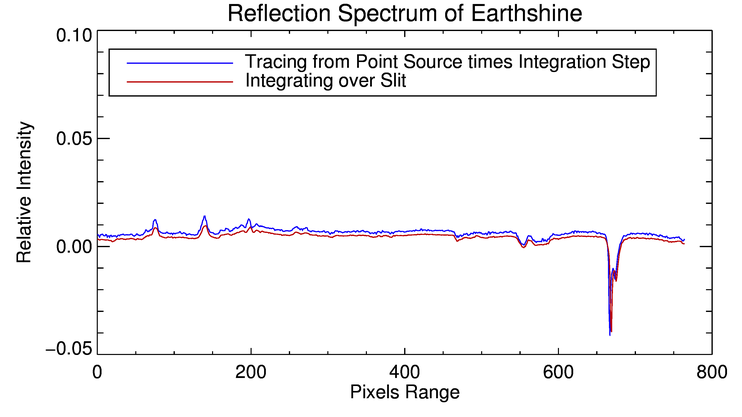
\includegraphics[scale=0.6]{plots/reflectivity0.png}
\caption{Earthshine reflectivity from method 1 and 2, scaled to each
other.}
\label{comparing2}
\end{center}
\end{figure}








\subsection{Absolute Spectra Calibration}
To obtain the absolute wavelengths of the Earthshine spectrum, we measure the
spectrum of a neon calibration lamp and compare it to the well-known wavelengths
of neon
transitions, see Fig. \ref{fig-neon}.

\begin{figure}[htb]
\begin{center}
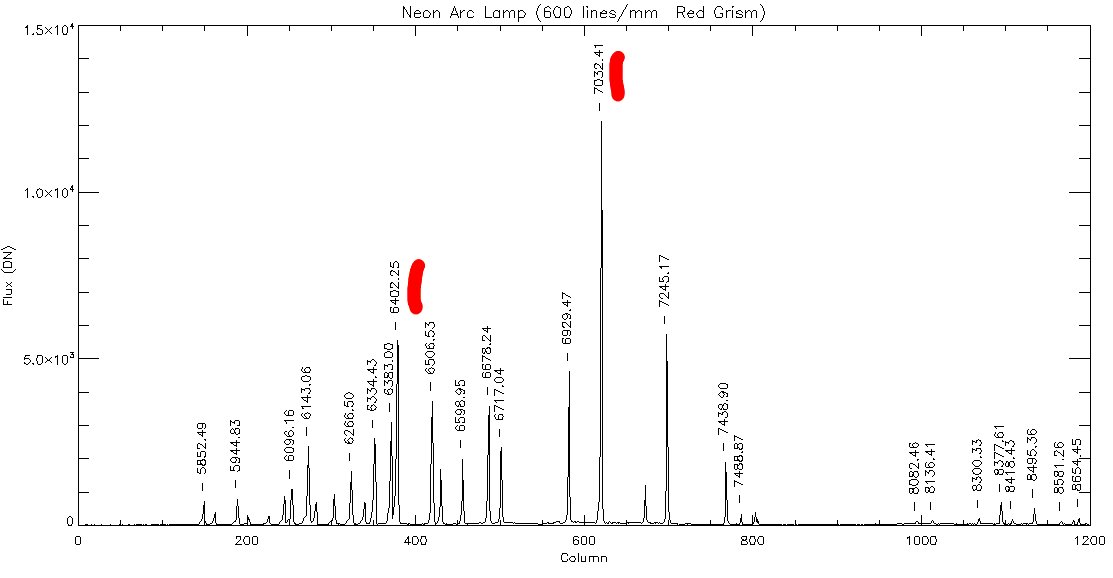
\includegraphics[scale=0.2]{figs/neon.jpg}
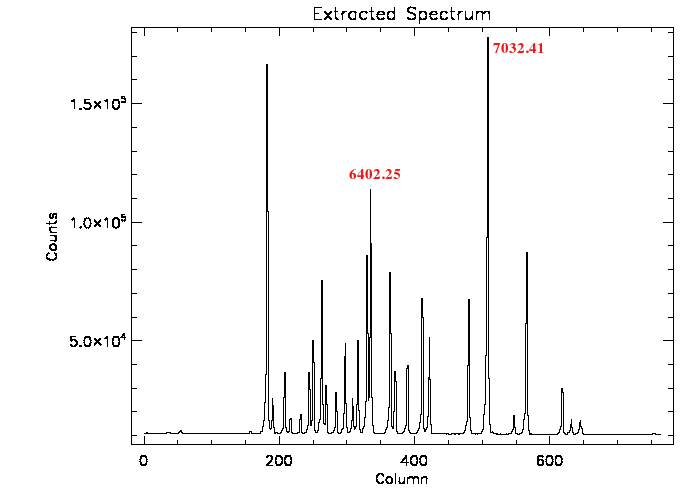
\includegraphics[scale=0.45]{plots/neon1.png}
\caption{Wavelength transitions of neon: (left) from the literature
\cite{neon-wave}, (right)  experimentally obtained.}
\label{fig-neon}
\end{center}
\end{figure}

We find the {\it $\lambda$/pixels scale dispersion} and we reduce the
Earthshine spectra from it.This results on the Earthshine spectra 
correlation to light wavelengths, \ie the reflectivity of the Earth.

\begin{figure}[htb]
\begin{center}
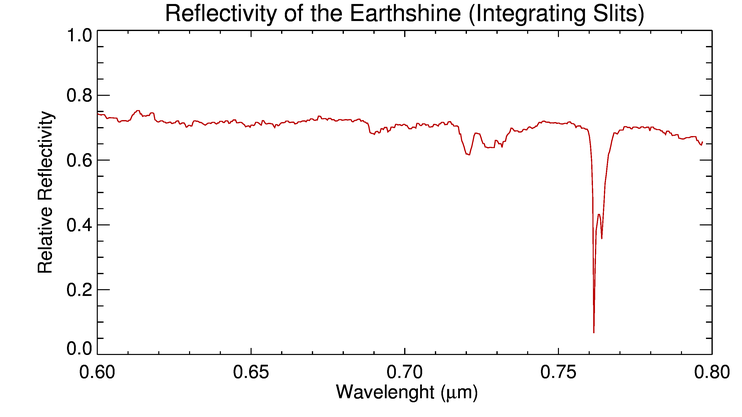
\includegraphics[scale=0.6]{plots/reflectivity2.png}
\caption{The Reflectivity of the Earth.}
\label{fig-es}
\end{center}
\end{figure}





